\section{Topologi}\label{sec:topologi}
Kort fortalt er topologi i prossmod kunsten å dele opp et system inn i mange små kontrollvolumer som ``snakker'' med hverandre. En topologi inneholder ingen matematiske uttrykk, men gir en oversikt over transport av impuls, varme og/eller masse mellom forskjellige kontrollvolum. Hvordan vi setter opp en topologi er best forklart gjennom et enkelt eksempel, se \cref{sec:topologi_figurer}. Men før vi går i gang må vi forklare et par konsepter.

\subsection{Intensive og ekstensive variabler}
\label{sec:ekstensive_intensive}
Forskjellen mellom en intensiv og en ekstensiv variabel er at en intensiv variabel forblir uforandret når man skalerer opp systemet. Ta eksempelvis et badekar med vann. Vi antar at det fulle badekaret rommer 60 liter, og temperaturen er 25 grader. Hvis vi øker størrelsen på badekaret vil ikke lenger det fulle volumet (den ekstensive variabelen) være 60 liter men temperaturen (den intensive variabelen) vil fortsatt være 25 grader. 

\begin{center}
    \textit{En intensiv variabel er uavhengig av størrelsen på systemet hvorav en ekstensiv variabel vil være avhengig av størrelsen. }
\end{center}

\textbf{Eksempel på intensive variabler:} Temperatur, trykk, tetthet, konsentrasjon, farge, kokepunkt.

\textbf{Eksempel på ekstensive variabler:} Volum, masse, mol, entalpi, entropi, varmekapasitet, 


\clearpage
\subsection{Figurer i en topologi}\label{sec:topologi_figurer}
Her kommer det en liste med forklaringer på de vanligste figurene du støter på når du skal lage en topologi i prossmod. For full liste, se ABC-heftet. 
\begin{table}[H]
    \centering
    \begin{tabular}{c|c}
        Lumped System/Kontrollvolum & \raisebox{-.5\height}{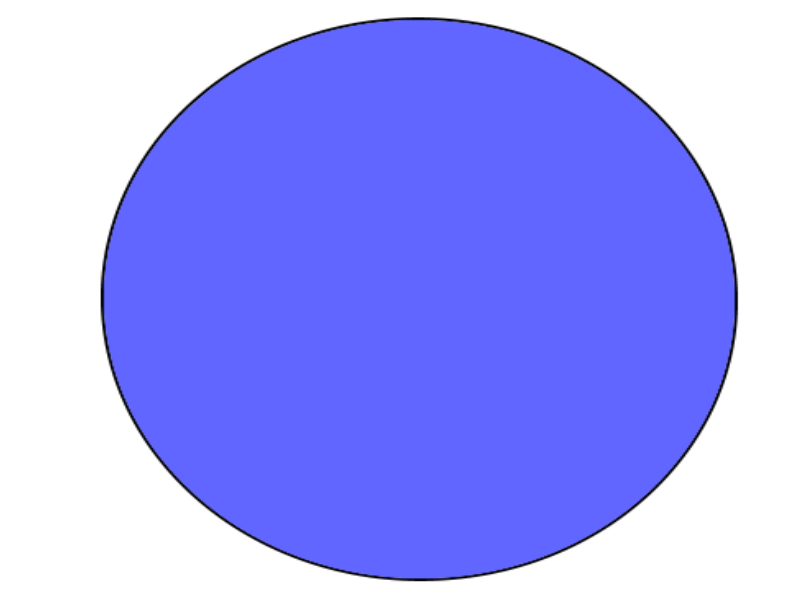
\includegraphics[scale=0.1]{Figures/Lumped.png}}\\
         Reservoar & \raisebox{-.5\height}{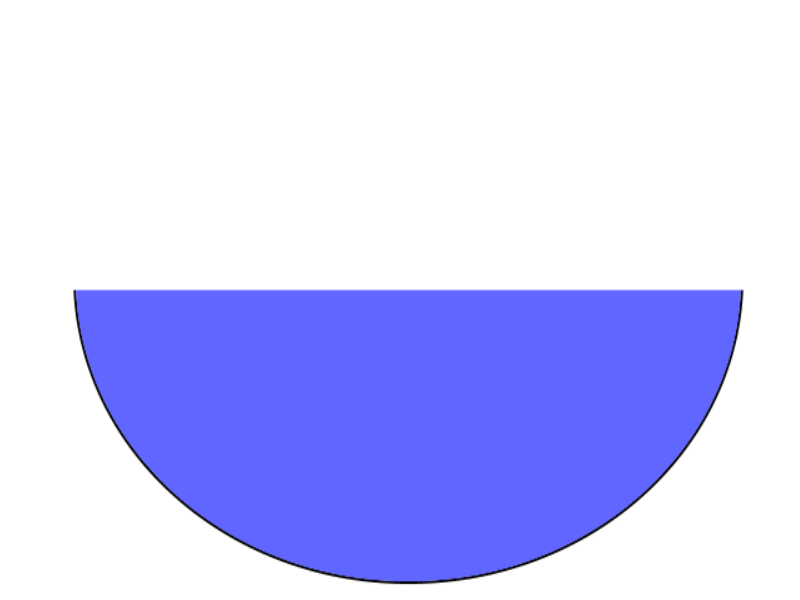
\includegraphics[scale=0.1]{Figures/Resavior.png}}\\ 
         Distributed system & \raisebox{-.5\height}{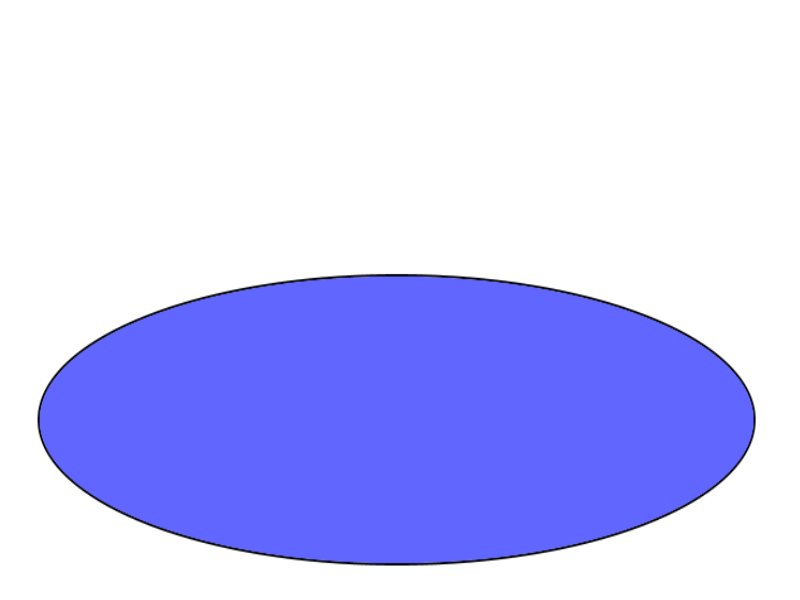
\includegraphics[scale=0.1]{Figures/Distributed.png}}\\
         Transport av masse & \raisebox{-.5\height}{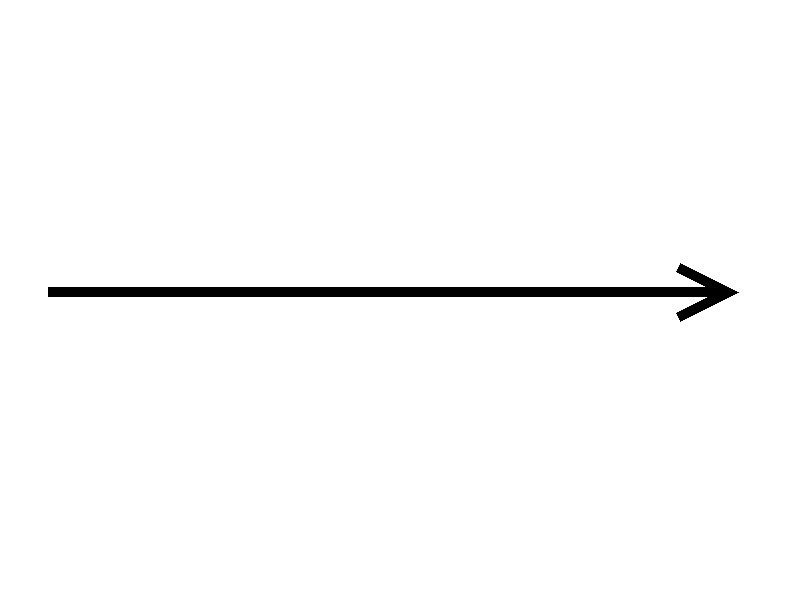
\includegraphics[scale=0.1]{Figures/mass_arrow.png}}\\
         Transport av varme (stråling, konduksjon) & \raisebox{-.5\height}{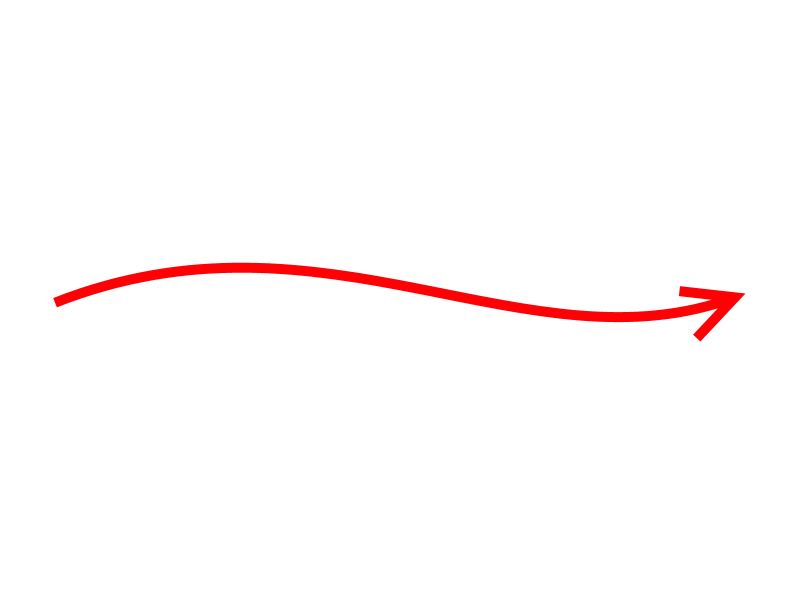
\includegraphics[scale=0.1]{Figures/Heat_arrow.png}} \\
         Transport av impuls (arbeid gjort fra et system)  & \raisebox{-.5\height}{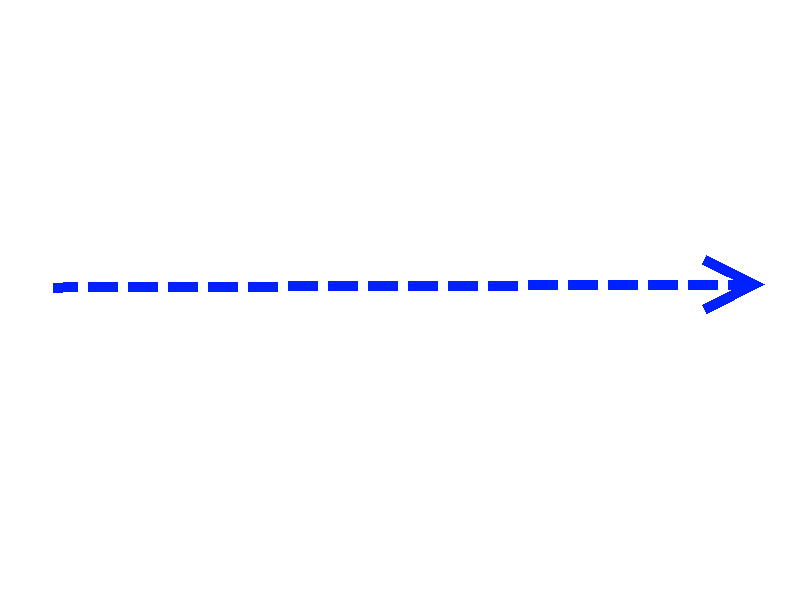
\includegraphics[scale=0.1]{Figures/Work_arrow.png}}\\
         Overflate uten kapasitet (event dynamic) & \raisebox{-.5\height}{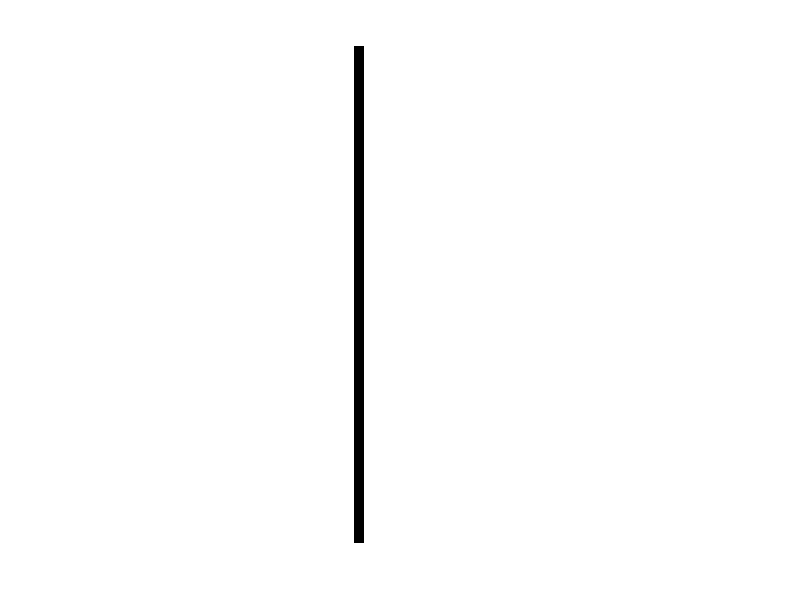
\includegraphics[scale=0.1]{Figures/surface.png}} 
    \end{tabular}
    \caption{De viktigste geometriske figurene vi finner i en topologi. For full liste, se ABC-heftet.}
    \label{tab:my_label}
\end{table}



\textbf{Lumped System}\\
Et lumped system representerer et volum/område for det fysiske systemet ditt. Ved å dele et stort system inn i mange små volumer kan vi få en grei forståelse av hvordan hver del av det store systemet kommuniserer. I et lumped system er det antatt at alle intensive variabler er isotrope. Det vil si at de intensive variablene er uavhengig av posisjon i systemet. Eksempelvis vil et målt trykk på 5 bar i volumet også være 5 bar alle andre steder i volumet. 

\textbf{Reservoar} \\
En stor menge som aldri går tom. Med andre ord vil et reservoar ha uendelig stor kapasitet i form av ekstensive variabler. Når det transporteres fra eller til et reservoar vil det ikke akkumuleres i reservoaret fordi reservoaret alt har uendelig mengde av den ekstensive variabelen. Alle intensive variabler i et reservoar er antatt å være konstante så et reservoar med 25 varmegrader vil forbli 25 varmegrader.

\textbf{Distributed systems}\\
Et distributed system er som et lumped system med unntak av at intensive variabler avhenger av hvor vi befinner oss i systemet (anisotropt system). Eksempelvis vil temperaturen i en badstue være høyere jo lengre opp i høyden du beveger deg. Av den grunn kan vi ikke lenger behandle volumet av en badstue som et lumped system. Vi må sette inn et distributed system. Merk at andre intensive variabler, som trykk og tetthet, kan være antatt konstante. Et distributed system kan være anisotrop i flere dimensjoner, men må minst være avhengig av en retning. Å modellere et distributed system er litt mer avansert, se \cref{sec:distributed}, men et lite partytriks er å bruke ``Sliced-salami'' metoden og dele et distributed system opp i flere mindre lumped systems. 


\textbf{Transportpiler}\\
Transportpiler er transport av ekstensive variabler fra et volum til et annet. Se \cref{sec:massetransport} for forklaring av modellering av transport. Merk at retningen på pilen er en referanse for modellen vår. Dette kan virke litt forvirrende, men det viktigste å vite er at når det transporteres fra et volum til et annet mot pilens retning, så må vi behandle transporten som negativ. Med andre ord er det ikke pilen i seg selv som bestemmer transporten, men retningen fungerer som en referanse når vi skal bestemme hvilken vei transporten går. 

\textbf{Overflater uten kapasitet}\\
Egentlig burde vi ha skrevet ``Event dynamic systems'', men det er litt forvirrende første gang man hører det. Det vi prøver å få fram er at vi har et system som ikke har mulighet til akkumulering siden hendelsen går så fort. Ta eksempelvis overflaten mellom vann og gass i fordampning av vann. Overflaten mellom væsken og gassen har ingen kapasitet og selve fordampningen skjer momentant. For å forklare at væske fordamper og blir til gass i topologien vår må vi ha med et event. I det tilfellet setter vi inn en rett strek, et event dynamic system. 

 
\subsection{Eksempel: Et basseng når det regner}
Tenk deg at sjefen din nettopp har fått installert et nytt fancy basseng i hagen og han har satt deg i oppgave å fylle opp bassenget med vann. Du ser på værmeldingen for morgendagen og oppdager at det er meldt 15 mm i timen. \enquote{Woho}, tenker du, \enquote{bassenget fyller seg opp av seg selv}. Før du begynner på regndansen funderer du på hvor mye vann som samler seg i bassenget på den tiden og du lurer på om du må fylle på med ekstra vann. Du bestemmer deg for å modellere bassenget og regnet som treffer det. Det første vi spør oss selv som ingeniører er: 

\begin{center}
    \textbf{1.} Hva ønsker jeg å finne ut av?
\end{center}

I dette tilfellet er det akkumuleringen av vann i bassenget. Vi ønsker å finne ut hvor mye vann som er samlet opp i bassenget etter en viss tid. Forklart matematisk så kan vi si mengde vann i bassenget ($m_{vann}$) er integralet av akkumulert vann i bassenget ($\dot{m}_{vann}$) fra start ($t_0$) til slutt ($t$)

\begin{equation}\label{eq:integral_over_time}
    m_{vann} = \int_{t_0}^{t}\dot{m}_{vann\,}dt 
\end{equation}

\cref{eq:integral_over_time} er nå modellen vår for bassenget. Vi integrer fra $t_0$ til en $t$ også vet vi hvor mye vann som er i bassenget vårt. Men vi har et problem, vi vet ikke hvor mye vann som akkumuleres i bassenget vårt; vi vet ikke hva $\dot{m}_{vann}$ er. Her trenger vi å sette opp en topologi. Vi må vite hvor mye vann som som kommer inn og hvor mye som går ut. Før vi kan tegne opp topologien vår må vi stille oss spørsmålet:

\begin{center}
    \textbf{2.} Hvilke antakelser tar jeg?
\end{center}

Nå som vi skal visualiserere systemet vårt gjennom en topologi må vi være klar over hvilke antakelser vi ønsker å gjøre i forkant av topologien. Et partytriks i prossmod er å alltid starte enkelt og så utvide topologien din ved å fjerne antakelser. I dette tilfellet vil muligens de viktigste spørsmålene være:

\begin{itemize}
    \item Lekker bassenget væske?
    \item Er det andre kilder av vann enn regnvann?
    \item Skal vi behandle all væske i bassenget som et system eller skal vi skille mellom vann og annet væske?
    \item Vil vann fordampe og gå ut fra bassenget?
    \item Skal vi bry oss om varmen i bassenget?
\end{itemize}

Først når vi er klar over hva vi neglisjerer og hva som ikke kommer fram i topologien vår kan vi skrive ned antakelsene og begynne å tegne. Her velger vi først å starte enkelt og anta at eneste kilde av væske er fra himmelen, all annen væske neglisjeres. Energibalanser ønsker vi ikke å modellere og vi antar at bassenget ikke lekker væske. 

\begin{center}
\textbf{3.} Tegn opp en topologi som reflekterer antakelsene
\end{center}

Basert på problemstillingen og antakelsene våre får vi en topologi med kun et lumped system og et reservoar. Merk at vi har valgt å se bort fra mye i starten for å få fram en enkel modell å jobbe med. Vi gjentar oss kanskje litt her, men det er fordi det er lett å forvirre seg selv. Tanken bak dette er at det er lettere å utvide en modell enn omvendt, og at det er mer strukturert å starte med det viktigste når man bygger en topologi fra scratch. 
\begin{figure}[H]
    \centering
    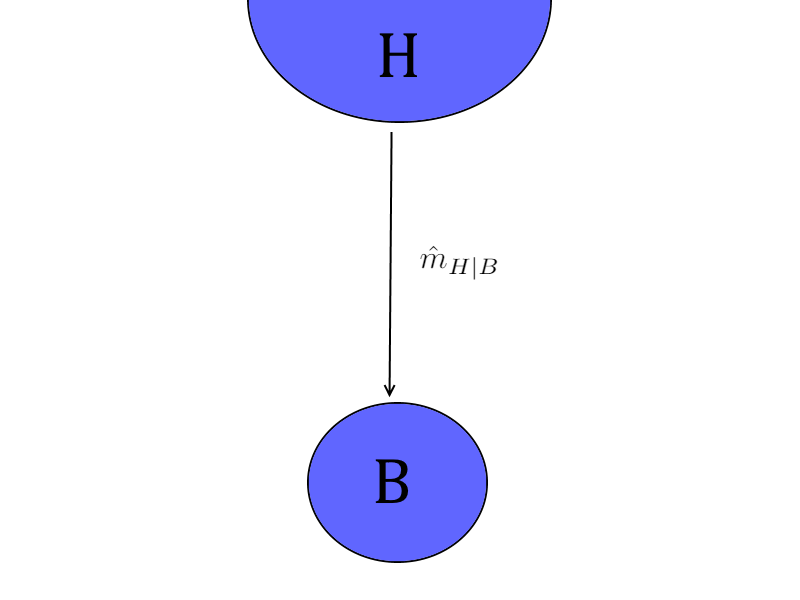
\includegraphics[scale=0.3]{Figures/Basseng1.png}
    \caption{Topologi av regnvann inn i et basseng, H representerer himmel og B representerer basseng.}
    \label{fig:topologi_enkel1}
\end{figure}

I \cref{fig:topologi_enkel1} ser vi representasjonen av massetransport fra H (himmel) til B (basseng). I denne topologien ser vi at all akkumulering av masse i B skyldes transporten fra H til B ($\hat{m}_{H|B}$). Nå som vi har en enkel modell kan vi vurdere hvorvidt vi skal utvide den eller ikke. Husk at en modell vil aldri være perfekt og det er bedre å ha en enkel modell som er god nok enn en vanskelig  modell som knapt forbedrer.  

\begin{center}
    \textbf{4.} Kan/bør jeg utvide topologien min?
\end{center}

 Topologien er på plass, livet er fint, men så kommer sjefen din og oppdager planen din om å la regnet gjøre arbeidet. Han fnyser av deg, men aksepterer  arbeidet ditt mot at du også skal ta hensyn til lekkasje og fordampingen av vann i bassenget. ``Fillern'' tenker du og hopper tilbake til arbeidet. Når vi utvider en modell er det viktig å gå tilbake på antakelsene og revurdere dem før vi utvider. For å få fram fordampningen og for å vise at bassenget vårt består av et volum av væske og et volum av gass setter vi opp to lumped systems med et event dynamic system mellom seg (overflaten). I tillegg antar vi at lekkasjen av væske skjer til bakken og at luften i bassenget forsvinner ut til omgivelsene.  
 
 \begin{figure}[H]
     \centering
     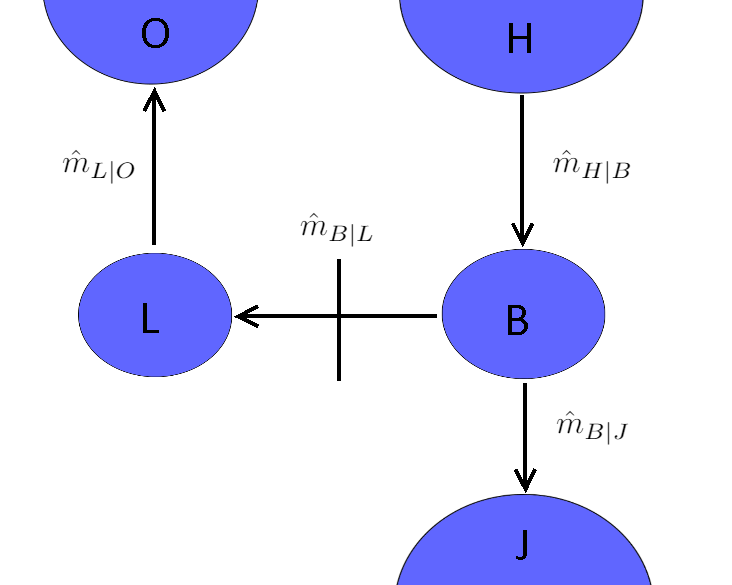
\includegraphics[scale=0.3]{Figures/Basseng2.png}
     \caption{Topologi av et basseng. H er en regnfull himmel, B er vannet i bassenget, L er luften i bassenget, O er luften i omgivelsene rundt bassenget, J er bakken.}
     \label{fig:basseng_vanskelig}
 \end{figure}

Den nye topologien er på plass og livet er nok en gang fint. Vi har laget en topologi hvor vi kan lage balanser rundt to volumer. Sjefen vår er ikke helt fornøyd og forventer at vi samtidig må ta hensyn til varmen i modellen vår. Vi sukker dypt, men etter litt tankegang kommer vi fram til en endelige topologi:

\begin{figure}[H]
    \centering
    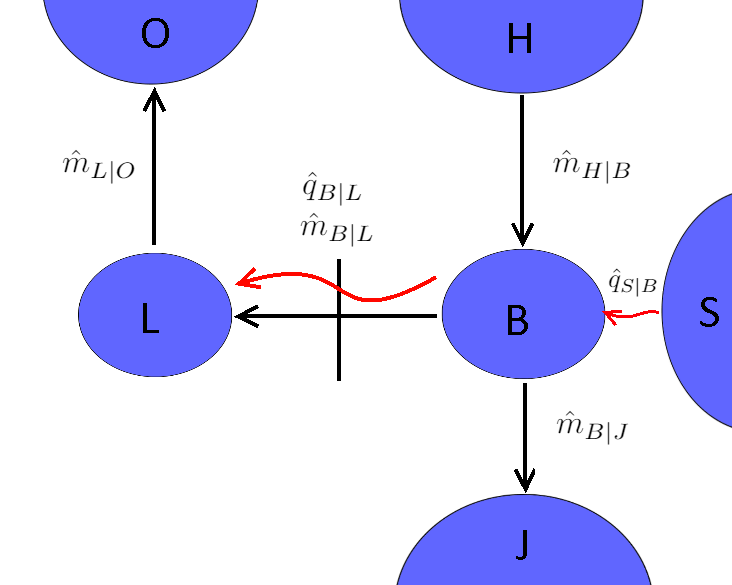
\includegraphics[scale=0.3]{Figures/Basseng3.png}
    \caption{Topologi av et basseng. H er en regnfull himmel, B er vannet i bassenget, L er luften i bassenget, O er luften i omgivelsene rundt bassenget, J er bakken, S er solen.}
    \label{fig:my_label}
\end{figure}
I denne topologien har vi antatt at solen er det eneste reservoaret av varme. Vi har neglisjert oppvarming av luften fra sola. Varmetransporten mellom B og L skyldes at hvis B skal fordampe kreves det energi i form av fordampningsentalpi. varmetransporten fra bassenget til jorda neglisjeres i denne modellen. Dette kan argumenteres med at temperaturforskjellen mellom bassenget og jorden er minmal så tapet av energi er ikke betydelig til modellen vår. Det er ganske forvirrende med modellering av varmetransport og du er ikke den eneste på IKP som synes det er vanskelig. Likevel er det en grei tommelfingerregel når det kommer til modellering a varmetransporten. Massetransport er all transport som følge av konveksjon mens varmetransport er all transport som følge av stråling og konduksjon, mer om dette i \cref{sec:konveksjon_konduksjon}. Heldigvis er vi nå ferdig med topologien vår. Vi leverer arbeidet vårt til sjefen som sier seg fornøyd og spanderer en Big Mac på oss. 

\begin{center}
    \textbf{5.} Ingen topologier er perfekte
\end{center}

Nå som vi har laget en topologi og ønsker å bruke den til å lage en matematisk modell for volumet i bassenget er det viktig å være klar over begrensninger ved modellen vår. For eksempel er det godt mulig at antakelsen vår om at isotropisk oppførsel for temperaturen i bassenget og luften ikke er en god antakelse. En mulighet kunne vært å sette inn et distributed system istedet, men det ville samtidig komplisere modellen vår. Ved å være klar over hva topologien ikke framstiller er vi også klar over hvilke begrensninger modellen vår har når vi bruker den. Å vite hva som er svakhetene ved en modell er essensielt siden du ikke har LF ute i arbeidslivet. 

\subsection{Oppsummert: Hvordan lage en topologi}
\begin{enumerate}
    \item Finn ut hva du ønsker å finne ut av. Er det modellering av masse, energi, impuls eller en kombinasjon?
    \item Hvilke antakelser er fornuftige? Start med det essensielle for problemet
    \item Tegn opp en topologi som reflekterer antakelsene
    \item Utvid topologien og modellen til du har en \enquote{god nok} representasjon av det fysiske systemet ditt
\end{enumerate}

\clearpage